\chapter{Layer 2 Scaling: Rollups}

\section{Introduction}
Rollups are a scaling solution used by the Ethereum community to increase throughput on the Ethereum Mainnet by moving computation and state-storage off-chain1. Rollups “roll up” a bunch of transactions into one and come in two basic forms: optimistic rollups and zero-knowledge rollups.\\
Optimistic rollups make the assumption that all of the rolled-up data is valid, and that nobody is trying to fool the blockchain by hiding spurious transactions within rollups. To protect against fraudulent transactions, optimistic rollup protocols allow people to contest bunk trades. The fraudulent transaction is submitted directly on the Ethereum network to check if it’s legit, and to settle the dispute.\\
Zero-knowledge rollups (also referred to as zk-rollups) work very differently. They rely on a piece of cryptography called a zero-knowledge proof, which allows someone to mathematically prove that a statement is true without disclosing additional information about that statement.\\
Rollups cut down on blockchain transaction costs by “rolling up” batches of transactions into a single one. They also speed things up: the rollup is very quick to perform and the Ethereum blockchain needs only to process a single transaction rather than many. That’s useful when Ethereum maxes out at around 15 transactions per second unassisted, see Figure \ref{fig:L14_f1}.
\begin{center}
	\begin{figure}
		\centering
		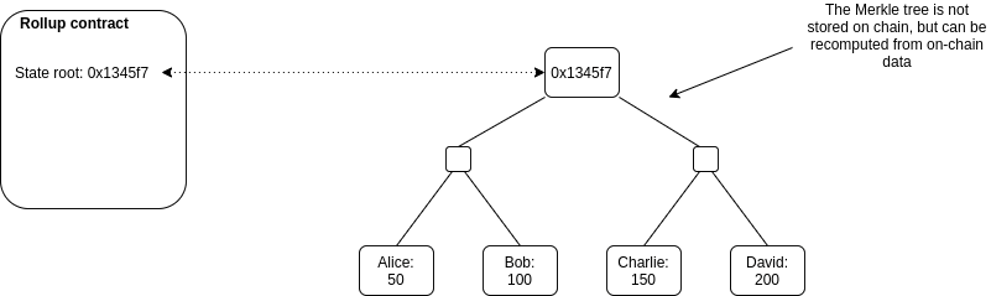
\includegraphics[width=0.8\linewidth]{Fig/14/F1}
		\caption{Rollups: A Scalable Solution for Ethereum - This diagram illustrates how Rollups execute transactions off-chain and report data on-chain in a compressed way, providing a scalable solution for Ethereum.
		}
		\label{fig:L14_f1}
	\end{figure}
\end{center}
\section{Transfer}
In a Rollup transfer, anyone can publish compressed data on-chain in a batch. This batch contains the pre-state, post-state, and compressed data. The diagram shows a Rollup contract connected to a State root with a dotted line. The State root is connected to four nodes representing Alice, Bob, Charlie, and David with solid lines. The nodes representing Alice, Bob, and Charlie are connected with a solid line, while the node representing David is connected with a dotted line. The text on the nodes reads “Alice $>$ Bob $>$ Alice $>$ Charlie $>$ Bob $>$ Charlie” and “David: compressed item. There is still enough data to determine how to update the state…”. This illustrates how Rollups can execute transactions off-chain while still maintaining the security and integrity of the blockchain, see Figure \ref{fig:L14_f2}.
\begin{center}
	\begin{figure}
		\centering
		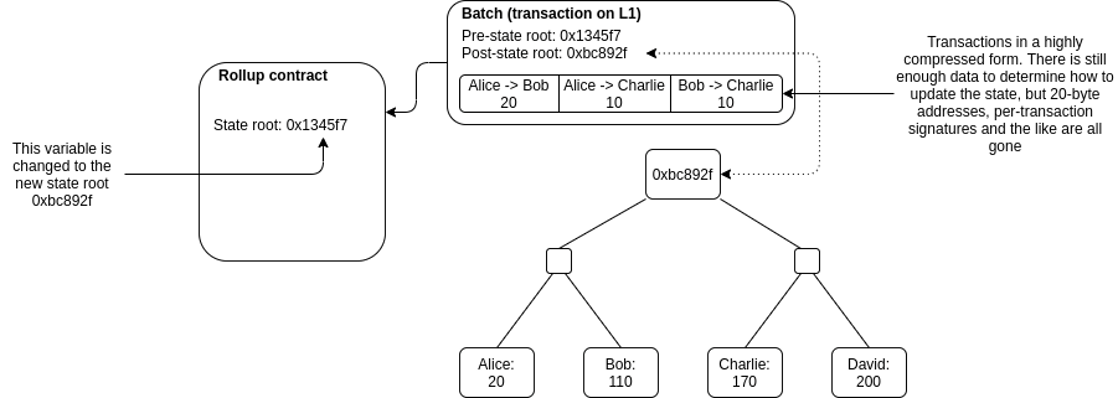
\includegraphics[width=0.8\linewidth]{Fig/14/F2}
		\caption{This diagram illustrates the concept of Rollups transfer in blockchain technology. It shows how anyone can publish compressed data on-chain, called a batch, which contains pre-state, post-state, and compressed data. The Rollup contract interacts with the state root, which in turn interacts with individual users such as Alice, Bob, and Charlie. The diagram also shows the balances of each user.
		}
		\label{fig:L14_f2}
	\end{figure}
\end{center}
For more information see Figure \ref{fig:L14_f3}, this diagram shows the process of publishing compressed data on-chain, referred to as a batch, which contains pre-state, post-state, and compressed data. The Rollup contract interacts with the state root, which in turn interacts with individual users such as Alice, Bob, and Charlie. The diagram also displays the balances of each user.
\begin{center}
	\begin{figure}
		\centering
		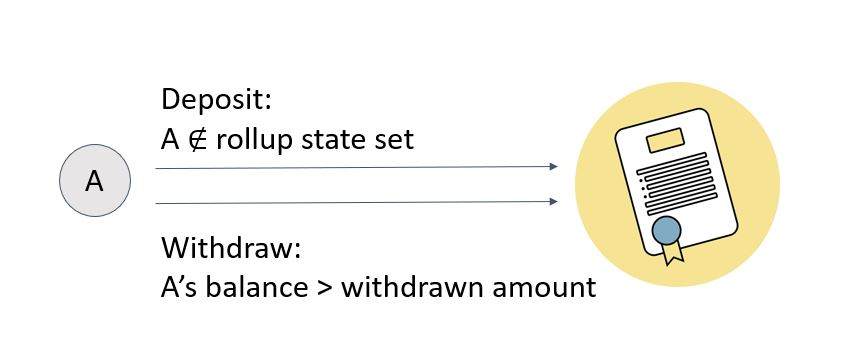
\includegraphics[width=0.8\linewidth]{Fig/14/F3}
		\caption{The image depicts a diagram that explains the concept of Rollups transfer in blockchain technology.
		}
		\label{fig:L14_f3}
	\end{figure}
\end{center}
\section{Optimistic Rollup}
Optimistic Rollup is a Layer 2 scaling solution designed to enhance the scalability of blockchain networks like Ethereum. It operates on the principle that the majority of transactions are valid and honest. By assuming transaction validity upfront and using fraud proofs to handle exceptions, Optimistic Rollup significantly increases the throughput and reduces transaction fees on the mainchain.
\subsection{Fraud Detection and Proofs}
Optimistic Rollups are a type of Layer 2 scaling solution for Ethereum that involves aggregating multiple transactions into a single block and submitting it to the Ethereum blockchain. This allows for faster and cheaper transactions.\\
Optimistic Rollups involve fraud proofs, which means that any user who sees an invalid state root can slash the aggregator by posting the valid state root. If a fraud proof is finalized, the chain is rolled back to the last valid state. This ensures the security and integrity of the system, see Figure \ref{fig:L14_f4}.\\
\begin{center}
	\begin{figure}
		\centering
		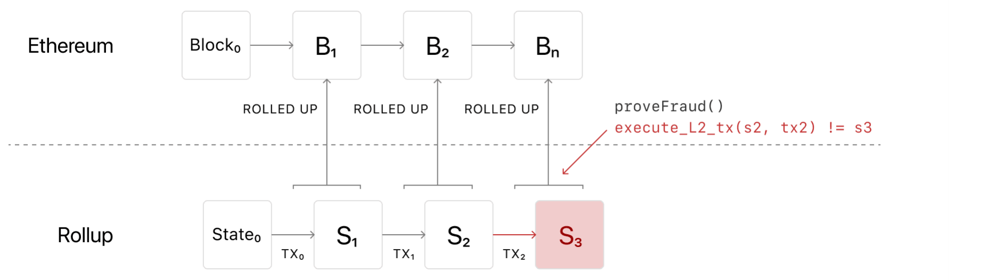
\includegraphics[width=0.8\linewidth]{Fig/14/F4}
		\caption{The blocks are labeled B1, B2, B3, etc., and the state transitions are labeled S1, S2, S3, etc. There is also a red arrow pointing to one of the blocks, indicating a fraud proof.
		}
		\label{fig:L14_f4}
	\end{figure}
\end{center}
\textbf{Fraud proof generation and verification with Merkle tree}\\ As we said before, a Merkle tree is a data structure that allows for efficient verification of the contents of large data sets. It is a tree in which every leaf node is labeled with the cryptographic hash of a data block, and every non-leaf node is labeled with the cryptographic hash of the labels of its child nodes. In the context of fraud proofs, a Merkle tree can be used to efficiently verify the validity of a state root by comparing it to the computed post-state root, see Figure \ref{fig:L14_f5}.
\begin{center}
	\begin{figure}
		\centering
		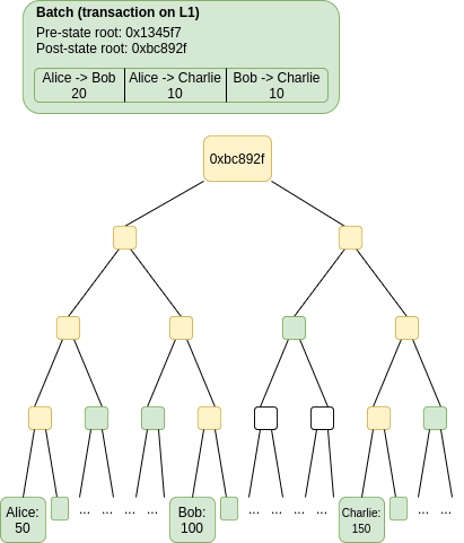
\includegraphics[width=0.8\linewidth]{Fig/14/F5}
		\caption{Batch transactions on L1: Keeping track of the numbers}
		\label{fig:L14_f5}
	\end{figure}
\end{center}
\textbf{Complexity of fraud proofs}
Fraud proofs are essential components of Optimistic Rollup and similar Layer 2 solutions. They serve as mechanisms to detect and correct invalid or fraudulent transactions without requiring the complete re-execution of these transactions on the Layer 1 (L1) mainchain. However, the traditional approach to verify fraud proofs can lead to substantial gas costs and overhead. The complexity can be broken down as follows:
\begin{enumerate}
	\item \textbf{Verify Fraud Proof Using a Verifier Contract:} The straightforward way to validate a fraud proof is by re-executing the disputed transactions on the Layer 1 chain. This involves interacting with a verifier contract deployed on the mainchain. The verifier contract checks the disputed transactions' correctness and enforces the correct state transition.
	\item \textbf{Optimism and Arbitrum: Methods to Reduce Overhead:} Optimism and Arbitrum are two innovative approaches that aim to mitigate the overhead associated with fraud proofs while maintaining the security and scalability benefits of Layer 2 solutions.
	\begin{enumerate}
		\item \textbf{Optimism:} Optimism introduces an optimistic execution model, where transactions are initially assumed to be valid and executed on the Layer 2 chain, adhering to the optimistic assumption. This eliminates the immediate need for costly re-execution on the L1 mainchain. Users can submit transactions with minimal fees and faster confirmation times.\\
		In the event of a dispute, users or validators can present fraud proofs to the mainchain to challenge the optimistic assumption. However, the key innovation is that the system incentivizes disputers to provide the full transaction data for re-execution only if a dispute is valid. This introduces a "dispute fee" mechanism, where the successful disprover is rewarded from the funds of the disproven transaction. This approach encourages the submission of fraud proofs only when necessary, reducing the overall overhead.
		\item \textbf{Arbitrum:} Arbitrum takes a similar approach to reduce overhead by utilizing a novel concept called "fraud proofs as data." Instead of requiring full re-execution on the mainchain, Arbitrum focuses on providing compact data that allows the mainchain to confirm the validity of transactions quickly and with minimal computation.\\
		Arbitrum's fraud proofs are designed to be computationally light and easily verifiable. They do not involve re-execution but rather rely on cryptographic proofs and aggregated state updates. This significantly reduces gas costs and overhead associated with dispute resolution.
	\end{enumerate}
	In summary, Optimism and Arbitrum address the complexity and overhead of fraud proofs by leveraging innovative execution models and cryptographic techniques. These approaches aim to strike a balance between security and efficiency, enabling Layer 2 solutions to provide scalability benefits without sacrificing the security of on-chain transactions.
\end{enumerate}
\subsection{Data Availability}
Data availability is a crucial aspect of Layer 2 solutions, as ensuring that all necessary transaction data is accessible is essential for the proper functioning of these systems. Here are some methods to address data availability:
\begin{enumerate}
	\item \textbf{All Compressed Transaction Data is On-Chain:} To ensure data availability, all compressed transaction data is stored on the main Ethereum chain. This approach guarantees that the necessary data for transaction execution is accessible to all participants. Storing the minimum required data on-chain allows Layer 2 solutions to operate effectively and maintain security.
	\item \textbf{Clever Compression Tricks:} Efficient data compression techniques can further optimize the storage and accessibility of transaction data on-chain.
	\begin{enumerate}
		\item \textbf{Use a Fixed Fee Level in Each Batch:} By employing a fixed fee level for transactions within each batch, the need to include the fee-related data for every transaction can be minimized. This helps reduce the overall data size and ensures data availability without overburdening the system with redundant fee information.
		\item \textbf{Replace the 20-byte Address with an Index:} Substituting the standard 20-byte Ethereum addresses with shorter indices can significantly reduce the data size of transactions. This optimization relies on maintaining an index-to-address mapping off-chain, which helps achieve efficient data storage while still allowing easy address resolution.
		\item \textbf{Use BLS Aggregate Signatures:} Utilizing BLS (Boneh-Lynn-Shacham) aggregate signatures allows multiple signatures to be combined into a single compact signature. This reduces the overall data size required to represent the signatures of multiple participants in a transaction batch, improving data availability and on-chain efficiency.
		\item \textbf{Write Transactions to Ethereum as Calldata:} Storing transaction data in Ethereum calldata, which is a more cost-effective data storage location compared to storage slots, can further optimize data availability. Calldata storage reduces gas costs and ensures efficient on-chain transaction data representation.
	\end{enumerate}
\end{enumerate}
In summary, addressing data availability in Layer 2 solutions involves storing compressed transaction data on-chain and implementing clever compression techniques to optimize the use of data storage. These approaches collectively ensure that the necessary transaction data is accessible, while simultaneously minimizing the associated storage costs and data overhead.
\subsection{Pros and Cons}
In this part, we provide a simple table to show pros and cons of this approach, see table \ref{table:L14_t1}.
\begin{table}[htbp]
	\centering
	\captionsetup{justification=centering}
	\caption[position=above]{Pros and cons of Optimistic Rollup}
	\begin{tabular}{|>{\centering\arraybackslash}p{8cm}|>{\centering\arraybackslash}p{8cm}|}
		\hline
		\textbf{pros} & \textbf{cons}\\
		\hline
		Offers massive improvements in scalability without sacrificing security.
		& Security model relies on at least one honest node executing rollup transactions and submitting fraud proofs.\\
		\hline
		Permissionless (anyone can force the chain to advance by executing transactions and posting assertions) & Users must wait for the one-week challenge period to expire before withdrawing funds back to Ethereum \\
		\hline
		Compatibility with EVM and Solidity allows developers to port Ethereum-native smart contracts to rollups & Rollups must post all transaction data on-chain, which can increase costs. \\
		\hline
	\end{tabular}
	\label{table:L14_t1}
\end{table}
\section{ZK Rollup}
Zero-Knowledge Rollups (ZK Rollups) are a Layer 2 scaling solution for blockchains that aims to improve the efficiency and scalability of transactions while maintaining a high level of security. ZK Rollups leverage the power of zero-knowledge proofs to achieve significant throughput improvements without compromising the security guarantees of the underlying blockchain.
\subsection{Validity Proof}
In ZK Rollups, a validity proof is generated using ZK-SNARKs to ensure that the state transition from the pre-state to the post-state has been executed correctly based on the provided transactions.\\
Components of the Validity Proof:\\
\begin{itemize}
	\item \textbf{C - State Transition Program:} The program C represents the state transition function or program. It describes how the blockchain state should change based on the given transactions. This program ensures that the pre-state is correctly updated to the post-state according to the specified rules.
	\item \textbf{x - Public Input:} The public input x consists of the pre-state and the post-state. It provides information about the initial state of the blockchain and the desired final state after processing the transactions.
	\item \textbf{w - Private Input:} The private input w comprises all the individual transactions that are being processed in the state transition. These transactions are kept private, and their details are used to generate the proof of the correctness of the state transition.
\end{itemize}
\textbf{Generating the Validity Proof:}\\
The ZK rollup coordinator, which is responsible for managing the Layer 2 solution, generates a SNARK proof $\pi$ using ZK-SNARK technology. This proof $\pi$ demonstrates that the coordinator knows the private transactions (input w) that lead to the correct update of the post-state from the pre-state according to the state transition program C.\\
By generating this validity proof, the ZK rollup coordinator provides cryptographic evidence that the state transition has been executed correctly, without revealing the specific details of the transactions. This proof can then be submitted to the main blockchain (Layer 1) for verification.\\
The use of ZK-SNARKs in ZK Rollups enables the creation of succinct and efficient proofs that demonstrate the integrity and validity of the state transition. It allows for substantial scalability improvements by reducing the computational load on the main blockchain while maintaining the security and trustworthiness of the entire system.
\subsection{Data availability}
While validity proofs in ZK Rollups ensure the correctness of state transitions and verify the knowledge of transactions, they do not inherently guarantee the availability of data related to those transactions on the blockchain. This is where the concept of "Transaction Summary" (TX summary) comes into play, see Figure \ref{fig:L14_f6}.\\
\textbf{What is Transaction Summary (TX Summary)?}\\
The Transaction Summary (TX summary) is a mechanism used to ensure the availability of transaction data on the blockchain. It provides a way to prove that the necessary data for processing transactions, such as input and output values, exists and can be reconstructed from the blockchain data. The TX summary acts as a complementary layer to the validity proofs, ensuring that all transaction details are accessible and can be verified by any party.\\
\textbf{Why is TX Summary Needed?}
\begin{enumerate}
	\item \textbf{Data Availability:}  The main purpose of TX summary is to guarantee the availability of transaction data. While validity proofs ensure the correctness of state transitions, they don't prove that the data used in those transactions is available to all participants. Without data availability, participants wouldn't be able to reconstruct and validate the state transitions themselves.
	\item \textbf{Resilience:} By including transaction data in a TX summary, the blockchain network becomes more resilient to data loss or unavailability. In cases where some transaction data is missing from the blockchain, participants can still reconstruct and validate the transactions using the TX summary.
	\item \textbf{Auditing and Verification:} The TX summary allows anyone to audit and verify the details of transactions. It provides a way for users, validators, and other stakeholders to independently verify that the transactions were executed correctly and that the associated data is present and retrievable.
	\item \textbf{Decentralization:} TX summary contributes to the decentralization of the data storage. Instead of relying on a single party or entity to store all transaction data, participants collectively ensure that the data is available and can be used for verification.
\end{enumerate}
In essence, the TX summary complements the validity proofs by ensuring that all necessary data for transaction execution and validation is available and can be reconstructed. It addresses potential issues related to data unavailability, enhances network resilience, and enables independent verification by participants.\\
It's important to note that different Layer 2 scaling solutions may implement TX summaries in different ways, and the specific technical details may vary. However, the underlying goal remains consistent: to ensure the availability of transaction data for proper verification and validation.
\begin{center}
	\begin{figure}
		\centering
		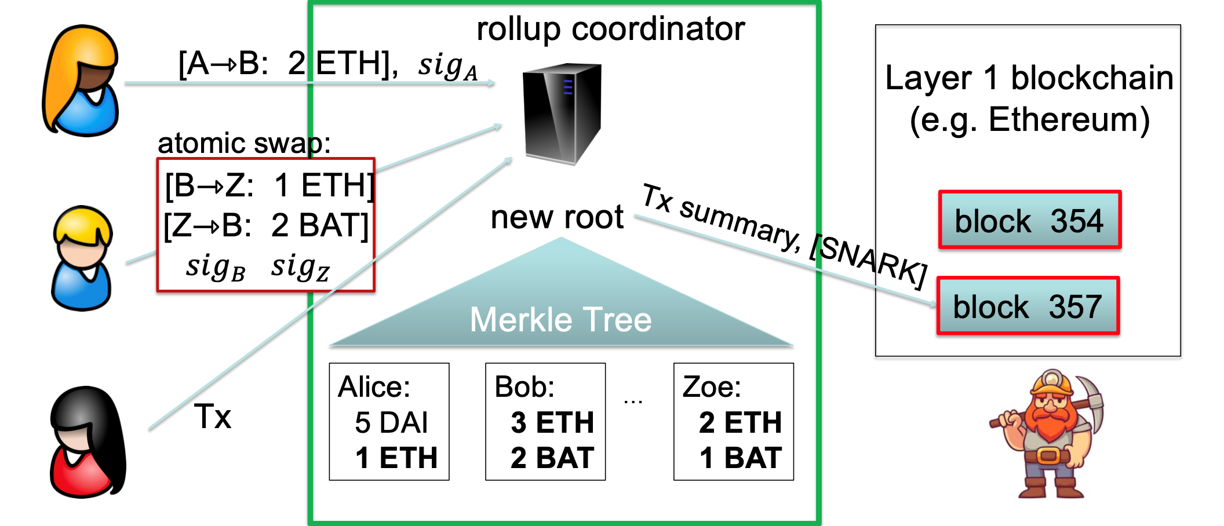
\includegraphics[width=0.8\linewidth]{Fig/14/F6}
		\caption{Data Availability: Ensuring the validity and authenticity of transactions with Merkle trees and snarks}
		\label{fig:L14_f6}
	\end{figure}
\end{center}
\subsection{zkSync vs. zkPorter}
These approaches focus on different methods of ensuring data availability and managing transaction summaries in a ZK Rollup setup. Here's a bit more detail on each approach:\\
\textbf{zkSync:}\\
\begin{itemize}
	\item \textbf{Transaction Summaries on Ethereum:} In the zkSync approach, transaction summaries are stored directly on the Ethereum blockchain. A crucial feature of zkSync is that Ethereum only accepts a transaction batch if it includes the summary of all transactions within that batch.
	\item \textbf{Reconstruction of L2 State:} Other coordinators can use the transaction summaries on the Ethereum blockchain to reconstruct the Layer 2 (L2) state. This ensures that all necessary data for transaction validation is available and can be verified independently.
	\item \textbf{Higher Ethereum Transaction Fees:} One downside of this approach is that storing transaction summaries directly on Ethereum can result in higher transaction fees, especially during periods of network congestion. This approach is more suitable for high-value assets or use cases where the higher cost is justified by the security and guarantees provided.
\end{itemize}
\textbf{zkPorter:}
\begin{itemize}
	\item \textbf{New Blockchain for Tx Data:} In zkPorter, the transaction data is stored on a new blockchain that is maintained by a set of staked coordinators. This new blockchain serves as an off-chain storage solution for transaction data.
	\item \textbf{Set of Staked Coordinators:} The new blockchain is secured and maintained by a group of coordinators who have staked tokens as collateral. These coordinators are responsible for ensuring data availability and correct execution of transactions.
	\item \textbf{Cost-Efficient Off-Chain Storage:} zkPorter benefits from cheaper off-chain storage compared to zkSync's on-chain approach. However, it may provide a slightly lower level of guarantee compared to zkSync due to the different security model.
	\item \textbf{Flexibility for Account Storage:} zkPorter allows customers to choose how coordinators store their account data, providing some flexibility in terms of data management.
\end{itemize}
Both zkSync and zkPorter represent innovative ways to address the data availability challenge in ZK Rollups. They offer different trade-offs in terms of transaction fees, security, and guarantees, allowing projects to choose the approach that best aligns with their specific use cases and requirements.
\subsection{EVM Compatibility}
EVM compatibility is a crucial aspect when considering the adoption of ZK Rollup solutions within the Ethereum ecosystem. Here's a brief overview of the challenges and some of the ongoing projects related to EVM compatibility in the context of ZK Rollups:\\
\textbf{Complexity and Proof Generation Challenge:} While ZK Rollups can efficiently handle simple computations like token transfers, more complex general-purpose computations that involve smart contracts are harder to prove within ZK-SNARK circuits. The process of creating proofs for complex computations can be resource-intensive and challenging.\\
\textbf{zkEVM. Ongoing Projects for EVM-Compatible ZK Rollups:}\\
\begin{enumerate}
	\item \textbf{Polygon (formerly Matic):} Polygon is working on implementing zkEVM, an EVM-compatible ZK Rollup solution. This aims to bring the benefits of ZK Rollups to Ethereum-compatible smart contracts, enabling scalable and low-cost execution of complex computations on the Ethereum network.
	\item \textbf{Scroll:} Scroll is a Layer 2 scaling solution that focuses on providing EVM compatibility for ZK Rollups. It aims to enable seamless integration of existing Ethereum smart contracts onto Layer 2 while maintaining compatibility with the Ethereum Virtual Machine.
	\item \textbf{zkSync:} zkSync, as mentioned earlier, is another project that is working on EVM compatibility. It seeks to allow Ethereum smart contracts to run on Layer 2 with the benefits of ZK Rollups, enhancing scalability and reducing transaction costs.
	\item \textbf{StarkWare:} StarkWare is a well-known name in the field of Layer 2 scalability. While they primarily focus on Stark-based solutions, which use a different zero-knowledge proof technology than ZK-SNARKs, they also contribute to EVM compatibility in Layer 2 solutions.
\end{enumerate}
These projects aim to overcome the challenges of implementing general-purpose EVM computations within ZK Rollup solutions. By providing EVM compatibility, they enable developers to migrate and deploy their existing smart contracts to Layer 2 environments, benefiting from improved scalability and reduced gas fees while maintaining the Ethereum programming model.
\subsection{zkEVM}
zkEVM (Zero-Knowledge Ethereum Virtual Machine) is a technology that brings the functionality of the Ethereum Virtual Machine (EVM) to a Layer 2 scaling solution, specifically a ZK Rollup. It achieves this by recreating existing EVM opcodes within a zero-knowledge proof system, enabling the execution of smart contracts off-chain while ensuring their correctness.\\
Here's a breakdown of how zkEVM works:\\
\begin{enumerate}
	\item \textbf{Recreating EVM Opcodes:} zkEVM implements a set of EVM opcodes within the context of zero-knowledge proofs. These opcodes represent the operations that smart contracts can perform on the Ethereum network, such as arithmetic computations, data storage, and control flow.
	\item \textbf{Computation and State Transition:} Similar to the EVM, zkEVM performs computation on given inputs within a smart contract. This computation results in a transition from one state to another. However, in zkEVM, these state transitions occur off-chain, reducing the computational and gas costs compared to on-chain execution.
	\item \textbf{Zero-Knowledge Proofs:} The key innovation of zkEVM is the generation of zero-knowledge proofs for every step in the program's execution. These proofs cryptographically verify that the computations performed in zkEVM are correct without revealing any sensitive information about the actual inputs or intermediate states.
	\item \textbf{Off-Chain Execution:} With zkEVM, smart contracts are executed off-chain within the Layer 2 environment. The zkEVM protocol creates and submits zero-knowledge proofs to the main Ethereum chain (Layer 1), providing cryptographic evidence of the validity of the computations performed off-chain.
	\item \textbf{Scalability and Efficiency:} By leveraging zero-knowledge proofs, zkEVM significantly reduces the amount of data that needs to be stored and verified on-chain. This results in improved scalability and reduced gas fees compared to directly executing smart contracts on the Ethereum mainnet.
\end{enumerate}
In summary, zkEVM allows developers to migrate their existing Ethereum smart contracts to a Layer 2 environment while maintaining compatibility with the Ethereum programming model. It achieves this by combining the familiar functionality of the EVM with the power of zero-knowledge proofs, enabling efficient and secure off-chain execution of smart contracts with cryptographic proofs of correctness.
\subsection{Pros and Cons}
In this part we provide a simple table to show pros and cons of this approach, see table \ref{table:L14_t2}.
\begin{table}[htbp]
	\centering
	\captionsetup{justification=centering}
	\caption[position=above]{Pros and cons of ZK Rollup}
	\begin{tabular}{|>{\centering\arraybackslash}p{4cm}|>{\centering\arraybackslash}p{4cm}|}
		\hline
		\textbf{pros} & \textbf{cons}\\
		\hline
		Short withdrawal delays	& Building EVM-compatible ZK-rollups is difficult due to complexity of ZK technology \\
		\hline
		Relies only on trustless cryptographic mechanisms for security & High cost on computing and verifying validity proofs \\
		\hline
		Only TX summaries on chain & Some proving systems (e.g., ZK-SNARK) require a trusted setup \\
		\hline
	\end{tabular}
	\label{table:L14_t2}
\end{table}
\section{Final Comparison}
In this part we bring a table to compare ZK and Optimistic Rollups approaches, see table \ref{table:L14_t3}.
\begin{table}[htbp]
	\centering
	\captionsetup{justification=centering}
	\caption[position=above]{ZK Rollups vs. Optimistic Rollups}
	\begin{tabular}{|>{\centering\arraybackslash}p{4cm}|>{\centering\arraybackslash}p{4cm}|>{\centering\arraybackslash}p{4cm}|}
		\hline
		\textbf{Property} & \textbf{Optimistic Rollups} & \textbf{ZK Rollups}\\
		\hline
		Fixed gas cost per batch & ~40,000 & ~500,000\\
		\hline
		Withdrawal period & ~1 week & Very fast \\
		\hline
		Complexity of technology & Low & High \\
		\hline
		Generalizability & Easier & Harder \\
		\hline
		Per-transaction on-chain gas costs & Higher & Lower \\
		\hline
		Off-chain computation costs & Lower & Higher \\
		\hline
	\end{tabular}
	\label{table:L14_t3}
\end{table}